\documentclass[]{article}
\usepackage{graphicx}
\usepackage{multirow}% http://ctan.org/pkg/multirow
\usepackage[utf8]{inputenc}
\usepackage[utf8]{inputenc}
\usepackage{graphicx,epstopdf,subfigure,mathtools,mathrsfs} 
%\usepackage[normalem]{ulem}
\PassOptionsToPackage{usenames,dvipsnames}{xcolor}
\usepackage[usenames,dvipsnames]{xcolor}
\newcommand{\cmt}[1]{\color{blue}#1\normalcolor}
\newcommand{\norm}[1]{\left\lVert #1 \right\rVert} 
\newcommand{\mat}[1]{\mathbf{#1}}
% notation
\newcommand{\bm}[1]{\mbox{\boldmath $ #1 $}}    % bold math mode
\renewcommand{\vec}[1]{\bm{#1}}                 % vector notation
\def\cddot{% two dots stacked vertically
  \mathbin{\vcenter{\baselineskip.67ex
    \hbox{\onedot}\hbox{\onedot}}%
  }}
  \usepackage{hyperref}
\hypersetup{
    colorlinks=false,
    pdfborder={0 0 0},
}

% Set the margins for 1" around
\setlength{\topmargin}{-0.5in}
\setlength{\oddsidemargin}{0.1in}
\setlength{\evensidemargin}{0.0in}
\setlength{\textwidth}{6.4in}
\setlength{\textheight}{8.9in}

\title{Parallel Immersed Boundary Method for Stokes Flow}
\author{Tristan Goodwill, Ondrej Maxian, and Anthony Trubiano}
\begin{document}
\maketitle

\section{IB Method}
We consider the immersed boundary method in the special case when the Stokes equations govern the fluid mechanics. That is, 
\begin{gather}
\label{eq:S1}
\mu \Delta \bm{u} - \nabla p + \bm{f} = \bm{0}, \\
\label{eq:S2}
\nabla \cdot \bm{u} = 0,
\end{gather}
where $\mu$ is the fluid viscosity, $\vec{u}$ is the fluid velocity, $p$ is the pressure, and $\vec{f}$ is an external forcing. We consider a periodic domain and use a spectral method to solve the equations. This involves taking a Fourier transform of $\bm{f}$, solving Eqs.\ \eqref{eq:S1} and \eqref{eq:S2} in frequency space for $p$ and $\bm{u}$, and then taking an inverse FT. 

In an IB-type formulation, the immersed structures (in our case fibers and/or spheres) are represented using a Lagrangian description, while the fluid quantities $\bm{u}$ and $p$ are represented on a collocated Eulerian grid. The IB method relies on a set of discrete interaction equations to obtain the force density on the grid from the Lagrangian force on the structures, and the velocity at the structures from the velocity on the grid. 

More specifically, let $\Gamma$ denote the Lagrangian domain, parameterized by material parameter $\bm{q}$ and $\Omega$ denote the fluid domain (a uniform grid with spacing $h$). The first equation for the interaction relates the fluid forcing $\boldsymbol{f}$ to the Force applied by the boundary $\boldsymbol{F}$ is
\begin{equation}
\label{eq:spread}
\bm{f}(\bm{x}) = \bm{\mathcal{S}} \bm{F}  = \int_{\Gamma}  \bm{F}(\bm{q},t) \delta_h (\bm{x} - \bm{X}(\bm{q},t))\, d \bm{q}  \approx \sum_{\bm{q}} \bm{F}(\bm{q},t) \delta_h (\bm{x} - \bm{X}(\bm{q},t)) \Delta \bm{q}. 
\end{equation}
Eq.\ \eqref{eq:spread} defines the \textit{spreading} operator $\bm{\mathcal{S}}$ and is used to calculate the force density $\bm{f}$ on the grid. $\delta_h$ is the classical 4 point regularized delta function of Peskin \cite{peskin2002acta}, which satisfies basic translation-invariant moment conditions. This function has the form
\begin{equation}
\delta_h(\bm{x}) = \frac{1}{h^3} \phi\left(\frac{x_1}{h}\right) \phi\left(\frac{x_2}{h}\right) \phi\left(\frac{x_3}{h}\right), 
\end{equation}
where $\phi(x)$ is some kernel with support on $-2 \leq x \leq 2$. See \cite{peskin2002acta} for more details for the derivation of the kernel. 


After spreading the force to the grid via $\bm{f}=\bm{\mathcal{S}}\bm{F}$, the Stokes equations are solved on the periodic domain via a spectral method. The structures are updated with the interpolated local fluid velocity, satisfying the no-slip boundary condition,
\begin{equation}
\label{eq:interp}
\frac{d \bm{X}}{dt} = \bm{U}(\bm{X}(\bm{q},t)) =\bm{S}^* \bm{u} = \int_{\Omega} \bm{u} (\bm{x},t) \delta_h(\bm{x}-\bm{X}(\bm{q},t))\, d\bm{x} \approx \sum_{\bm{x}} \bm{u}(\bm{x},t) \delta_h (\bm{x} - \bm{X}(\bm{q},t)) h^3. 
\end{equation}
In Eq.\ \eqref{eq:interp}, we have defined the \textit{interpolation} operator $\bm{S}^*$ that acts on the fluid grid velocity $\bm{u}$ to obtain the velocity at the structure points $\bm{U}$. 

To summarize, the IB method is composed of the following steps
\begin{enumerate}
\item Given a configuration of the Lagrangian structures $\bm{X}$, compute the force $\bm{F}$ on the structure points. 
\item Spread the force to the grid via Eq.\ \eqref{eq:spread}
\item Solve the fluid equations on the grid via a spectral method. 
\item Interpolate the velocity from the grid to the structure via Eq.\ \eqref{eq:interp}
\item Evolve the structure positions via a forward Euler method. 
\end{enumerate}

\subsection{Programming aspects}
In this section, we focus on how we parallelized each of the steps 1-5. 

\subsubsection{Force computation}
In most cases, the force applied by the boundary is based on some local deformation of the immersed structure, for example from stretching and bending. Such a force can be computed point by point and is therefore embarrassingly parallel. In fact, the force computation is generally so fast (relative to the other routines) that it makes little difference whether it is done in parallel or serial. 

\subsubsection{Force spreading}
The spreading computation, Eq.\ \eqref{eq:spread} is not trivial to parallelize because multiple Lagrangian points exert force on the same grid point. This fact and the unstructured nature of the immersed boundary mean that attempting to parallelize this interaction in a shared-memory fashion leads easily to race conditions and must be done carefully. We adopt the scheme of McQueen and Peskin \cite{mcqueen} shown in Fig.\ \ref{fig:parspread}. We divide the grid into columns that run along the $z$ direction. Each column is assigned a number, and the boundary points are ``binned'' into the columns using a linked list (there is an array called ``first'' which has the index of the first point in each column, and an array called ``next'' which has the index of the next point in each column or 0 if the last point has already been selected). 

After the points are assigned bins, we observe that bins whose boundaries are at least 3 mesh-widths apart will not interact with the same grid points, since the support of the $\delta_h$ function is 2 mesh-widths. We can therefore spread all of the points in these bins (colored in black in Fig.\ \ref{fig:parspread}) in parallel. We refer to this operation as the spreading of one grid ``color.'' We then move the colors over by one and repeat. In all, there are sixteen colors, which are looped over in serial. Within each color, we loop over the bins in parallel and increment the array for forces on the grid accordingly. 

\subsubsection{Fluid solver}
The fluid solver exploits the periodic nature of our domains and the fact that solving for each Fourier mode of the fluid velocity and pressure is uncoupled and can be done algebraically. Thus the solve in Fourier space is embarrassingly parallel and fast. In order to solve in Fourier space, we must take Fourier transforms of each component of the force and take inverse Fourier transforms of the fluid velocities and pressures, totally 7 Fourier transforms. To do these transforms, we call the FFTW library, which is a highly optimized FFT library that provides options for acceleration using OpenMP and MPI parallelization. We explored both of these options.

\subsubsection{Interpolation}
After the velocity on the grid is computed, we need to use Eq.\ \eqref{eq:interp} to obtain the fluid velocities at each boundary point. Fortunately, this operation is embarrassingly parallel as boundary points are independent. The array of velocities on the grid comes from the fluid solver and only needs to be accessed (but not modified) to determine the velocity at each point. We can therefore loop over the points in parallel to obtain their velocities. 

\subsubsection{Evolving the structure}
We evolve the time structure using Forward Euler, though any other explicit ODE method could be used. Once the velocity of each point on the structure is known from interpolation, we can loop over the points in any parallel manner to get their new position. 

\begin{figure}
\centering     
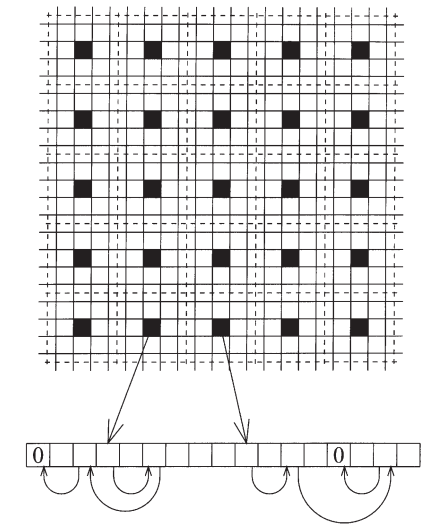
\includegraphics[width=70mm]{PeskinMcQueen.png}
\caption{Spreading the Lagrangian force to the grid in parallel (taken from \cite{mcqueen}). As in \cite{mcqueen}, we divide the 3D grid into columns and bin the points using a linked list (shown at bottom). There are 2 arrays, one which gives the location of the first point in each bin, and one which gives the location of the next point from the previous point (or 0 if there is no next point). We can then divide the columns into 6 ``colors,'' one of which is shown in black. Within each color, the points in the columns do not interact on the grid, since the support of the $\delta_h$ function is 2 mesh widths in either direction. We can therefore loop over the colors in serial, and the bins within each color in parallel. }
\label{fig:parspread}
\end{figure}


\section{Results}
In this section, we consider 2 possible scenarios for the immersed objects. The first is that the objects are a set of randomly distributed \textit{points} with random forces on them. This seems to us to be the best case scenario for parallelization because the boundary points are not coupled to each other and likely to be more evenly distributed between colours. As a more realistic case, we consider a system of \textit{fibers}, where the fiber points are connected to each other locally (this should make the spreading routine more difficult to parallelize as boundary points will cluster into bins, leaving other bins empty). We conducted a strong scaling study and a weak scaling study for each component of our scheme and the results are included below.

\subsection{Strong scaling}
We consider 2 cases for the strong scaling study: $10^6$ particles with random forces and 8000 fibers (with 128 points each) that are initially curved. In all cases, the grid size $256^3$ was chosen so that the serial spreading, fluid solve, and interpolation times are approximately equal. We note that these are large problems, and are therefore represent a near-optimal case for parallelization. 

We concern ourselves with the time to \textit{spread} the force to the grid, \textit{solve} the fluid equations on the grid, and \textit{interpolate} back to evaluate the velocities at the points (included in this is the time to take a forward Euler step to update the points). We have run this test on \texttt{crunchy1} and results were averaged over 2 trials. 

Fig.\ \ref{fig:Strong} shows the results of the strong scaling study. We see that, for both fibers and particles, interpolation scales extremely well with the number of cores. In fact, as we move from 1 to 32 cores, we obtain almost ideal scaling of interpolation. Spreading is slightly more complex; while the computation time does drop as we increase the number of cores, it is slow (relative to ideal scaling). This is likely due to memory bounds, as the array ``first'' must be accessed, even for empty bins. Furthermore, part of the force computation is to bin the points, which we currently do in serial because the arrays ``first'' and ''next'' depend on results from prior points. We are therefore bound Amdahl's law. This bound could be reduced by parallelizing the binning of points that are well separated. That said, we have still reduced the time for spreading by about an order of magnitude from 1 to 64 cores. 

Finally, the fluid solve is the slowest operation. This is to be expected, as it is the most complicated routine in the algorithm. The parallelization in the fluid solve comes from evaluating the 3D FFT of the forces, and subsequent inverse FFTs, in parallel using the FFTW3 library. However, this is far from the only step in the fluid solve. The creation, destruction, and execution of the FFTs are performed in serial, as well as array initialization and the algebraic computations necessary for the Poisson solve in Fourier space. Amdahl's law takes effect here, which is why the fluid solve seems to reach a lower bound in its computation time. 

In order to show that it is possible to have a better scaling fluid solve system, we implemented an MPI-version of the fluid solve. As we only have implemented shared memory interpolation and spreading routines, we do the fluid-structure interaction in shared memory, scatter the forces to several processes, use our MPI-based fluid solver, and then gather the fluid velocity. Because of this process, we report three times, the time for the fluid solve alone, the time for the fluid solve and FFTs and the time that includes scattering and gathering. Fig.\ \ref{fig:StrongMPI} shows the results of this strong scaling test. In this plot we see that ideal scaling is not achieved for anything except for the embarrassingly parallel solve in Fourier domain, and the overall fluid solve does scale reasonable well as we increase the number of processes. The non-ideal scaling of the Fluid solve is likely due to the increased amount of communication required for larger numbers of processors.

Overall, the MPI-based fluid solver scaled better than the OpenMP solver because they attempt to parallelize the Fourier transforms in different ways. The MPI-based scheme computes the independent Fourier transform of different rows in parallel, whereas the OpenMP-based scheme attempts to use multiple processes to accelerate a single Fourier transform at a time, which will be slower because of the tree structure of the FFT algorithm.
\begin{figure}
\centering     
\subfigure[$10^6$ particles]{\label{fig:SP}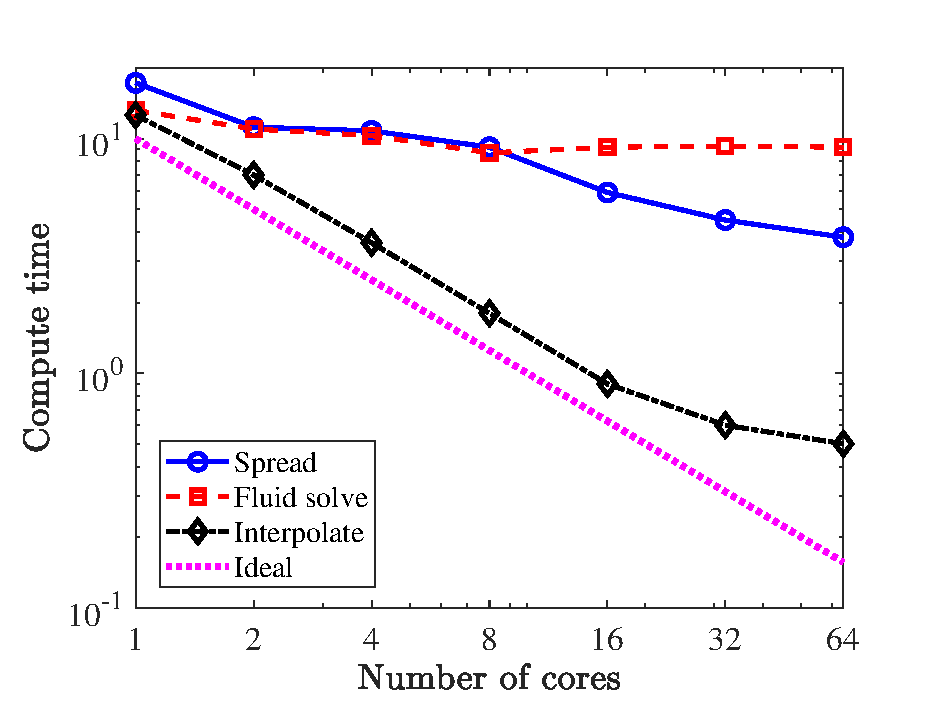
\includegraphics[width=70mm]{StrongScPoints.eps}}
\subfigure[8000 fibers]{\label{fig:SF}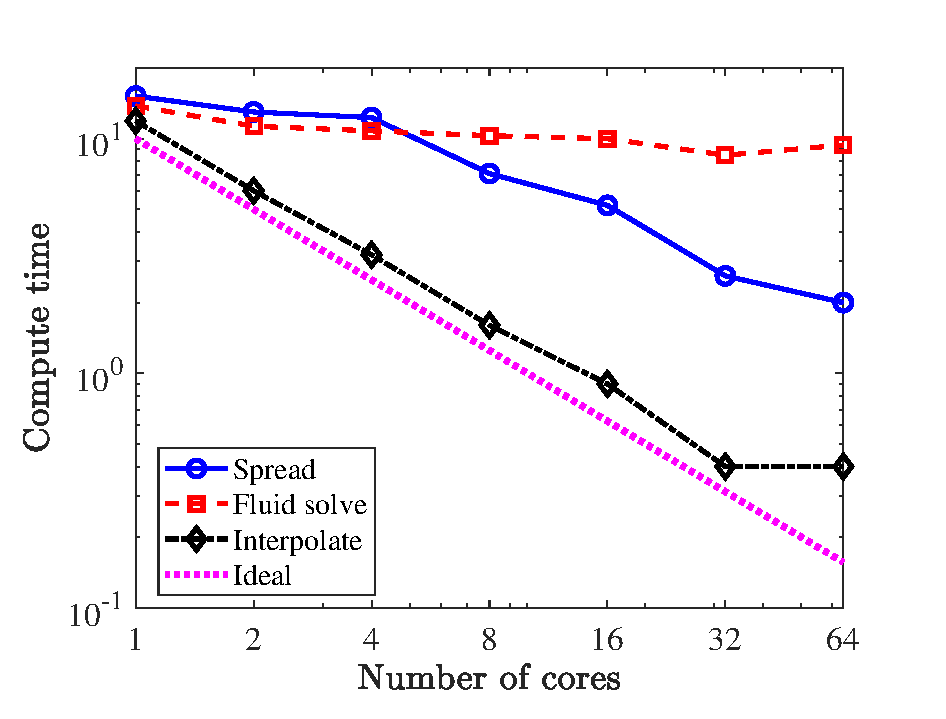
\includegraphics[width=70mm]{StrongScFibers.eps}}
\caption{Time to spread forces (blue circles), fluid solve (red squares), and interpolate velocities (black diamonds) for (a) $10^6$ fluid markers and (b) 8000 fibers of 128 markers each as a function of the number of processors. Ideal scaling is also shown, and interpolation is observed to scale best, while the fluid solve barely scales, indicating memory bounds. }
\label{fig:Strong}
\end{figure}
\begin{figure}
	\centering     
	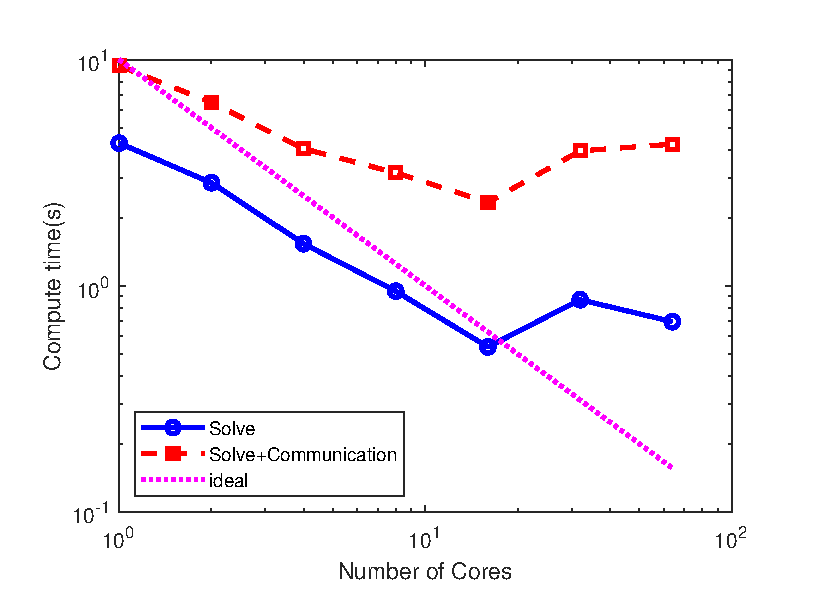
\includegraphics[width=70mm]{StrMPI.eps}
\caption{Time to solve the fluid equations using the MPI-version of FFTW on \texttt{crunchy3} (which has 32 cores) on a $256^3$ grid. The plot shows both the time taken to solve the equations in Fourier space(blue circles), the time taken to solve the fluid equations and compute FFTs (black diamonds) and the time taken to solve and communicate data (red squares). We see that good, though not ideal scaling is observed overall, when the number of processes is smaller than number of cores on \texttt{crunchy3}}
\label{fig:StrongMPI}
\end{figure}
\subsection{Weak Scaling}

\begin{figure}
	\centering     
	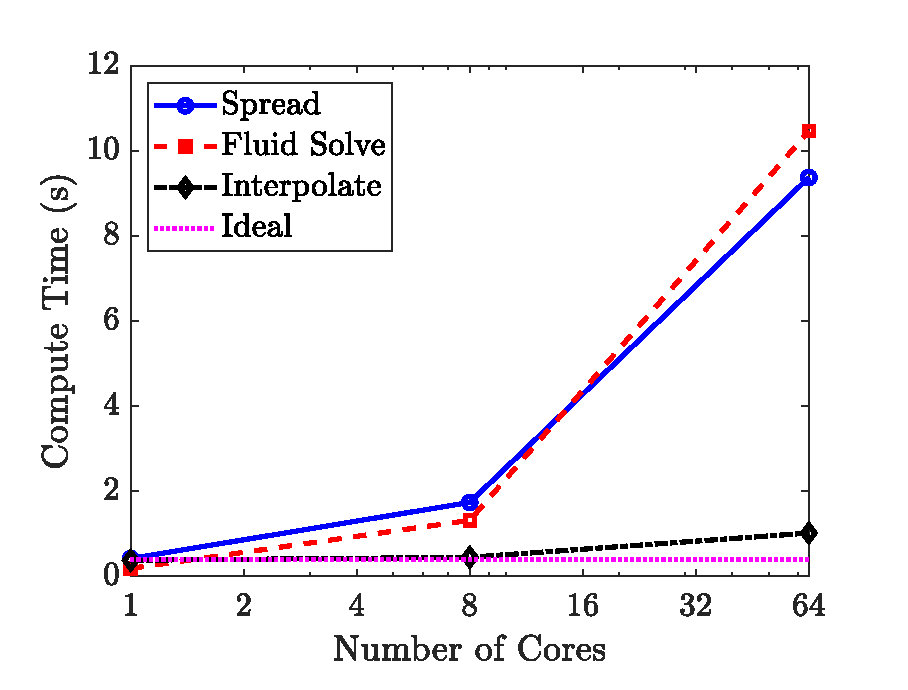
\includegraphics[width=70mm]{WeakScFibers.eps}
\caption{Weak scaling study for the 3 main routines of the immersed boundary method; spread, fluid solve, and interpolation. The initial test with 1 core uses a $64\times64\times64$ grid with 1000 fibers.  The number of cores is multiplied by $8$ in each successive test, in which the grid size is doubled. Interpolation scales well, remaining nearly constant in compute time, whereas spreading and solving do not scale well.}
\label{fig:Weak}
\end{figure}
\begin{figure}
	\centering     
	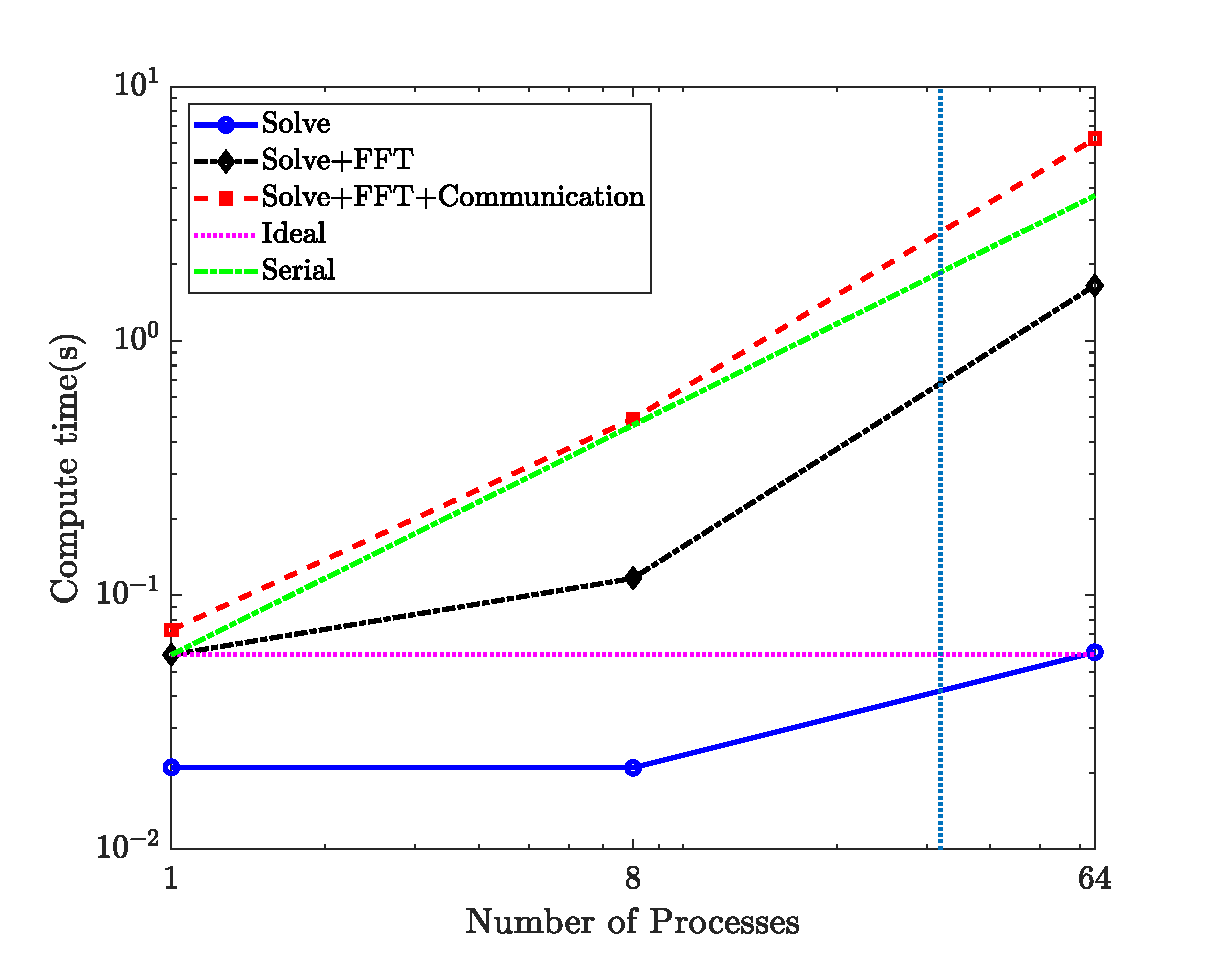
\includegraphics[width=70mm]{WeakMPI.eps}
\caption{Weak scaling study for the MPI version of the fluid solve. The initial test used a $64^3$ grid and in each successive test, the total number of grid points and processes was multiplied by 8. We see that the Fourier-space solve (blue circles) scales well for a number of processors less than the number of cores on \texttt{crunchy3}; the total fluid solve scales decently; and the communication scales as poorly as a serial code.}
\label{fig:WeakMPI}
\end{figure}
For our weak scaling study, we restrict ourselves to the case of immersed fibers. We start by using a single core with 1000 fibers on a grid of size $64^3$. We then want to make sure every processor does the same amount of work as we increase the problem size. We do this by properly scaling the number of Lagrangian points that need to be worked on. If the grid size is doubled, the number of grid points increases by a factor of 8. We then need $8$ times as many points on the fibers (to maintain the $2$ points per mesh-width heuristic). Thus, we should use $8$ time as many cores every time the grid size is doubled. 

Fig.\ \ref{fig:Weak} shows the results of the weak scaling study, performed on \texttt{crunchy1}. As before, the interpolation step scales nearly ideally, taking an almost constant amount of time for the increasing problem size. Spread and interpolate do not scale nearly as well, taking $8$ to $10$ times longer, despite having to do a similar amount of work. This is not surprising for the fluid solve, as we previously saw this step was the bottleneck in the strong scaling study. However, the spread scales just as poorly as the fluid solve in the weak sense, despite the noticeable speed ups in the strong scaling study. This is likely due to the fact that when the problem size increases, we do not spread the work evenly across processors, as points are concentrated in the same area. It is likely that there is a large load imbalance here, as well as memory effects mentioned previously. 







\newpage
\bibliographystyle{plain}

\bibliography{IBBib}
\end{document}
